\documentclass{../mcsslides}

\slidetitle{Практика 2: Объектно-ориентированное проектирование}{13.09.2022}

\begin{document}

    \begin{frame}[plain]
        \titlepage
    \end{frame}

    \section{Абстракция}

    \begin{frame}
        \frametitle{Абстрактные типы данных}
        \begin{itemize}
            \item \mintinline{java}|currentFont.size = 16| --- плохо
            \item \mintinline{java}|currentFont.size = PointsToPixels(12)| --- чуть лучше
            \item \mintinline{java}|currentFont.sizeInPixels = PointsToPixels(12)| --- ещё чуть лучше
            \item \mintinline{java}|currentFont.setSizeInPoints(sizeInPoints)| \newline
                    \mintinline{java}|currentFont.setSizeInPixels(sizeInPixels)| --- совсем хорошо
        \end{itemize}
    \end{frame}

    \begin{frame}[fragile]
        \frametitle{Пример плохой абстракции}
        \begin{minted}{java}
public class Program {
    public void initializeCommandStack() { ... }
    public void pushCommand(Command command) { ... }
    public Command popCommand() { ... }
    public void shutdownCommandStack() { ... }
    public void initializeReportFormatting() { ... }
    public void formatReport(Report report) { ... }
    public void printReport(Report report) { ... }
    public void initializeGlobalData() { ... }
    public void shutdownGlobalData() { ... }
}
        \end{minted}
    \end{frame}

    \begin{frame}[fragile]
        \frametitle{Пример хорошей абстракции}
        \begin{footnotesize}
            \begin{minted}{java}
public class Employee {
    public Employee(
            FullName name,
            String address,
            String workPhone,
            String homePhone,
            TaxId taxIdNumber,
            JobClassification jobClass
    ) { ... }

    public FullName getName() { ... }
    public String getAddress() { ... }
    public String getWorkPhone() { ... }
    public String getHomePhone() { ... }
    public TaxId getTaxIdNumber() { ... }
    public JobClassification getJobClassification() { ... }
}
            \end{minted}
        \end{footnotesize}
    \end{frame}

    \begin{frame}[fragile]
        \frametitle{Ещё один пример абстракции}
        \begin{columns}
            \begin{column}{0.32\textwidth}
                \begin{minted}{java}
public class Point {
    public double x;
    public double y;
}
                \end{minted}
            \end{column}
            \begin{column}{0.05\textwidth}
                vs
            \end{column}
            \begin{column}{0.65\textwidth}
                \begin{minted}{java}
public interface Point {
    double getX();
    double getY();
    void setCartesian(double x, double y);
    double getR();
    double getTheta();
    void setPolar(double r, double theta);
}
                \end{minted}
            \end{column}
        \end{columns}
    \end{frame}

    \begin{frame}
        \frametitle{Структуры против объектов}
        \begin{itemize}
            \item Объекты скрывают свои данные за абстракциями и предоставляют функции для работы с ними
            \item Структуры раскрывают данные и не имеют осмысленных функций
        \end{itemize}
        \vspace{3mm}
        \begin{itemize}
            \item Процедурный код позволяет легко добавлять новые функции без изменения существующих структур данных
            \item Объектно-ориентированный код, напротив, упрощает добавление новых классов без изменения существующих функций
        \end{itemize}
        \vspace{3mm}
        Пример --- списки в F\#. Тип list имеет 7 методов, тип Collections.List --- больше 60
    \end{frame}

    \begin{frame}[fragile]
        \frametitle{Уровень абстракции (плохо)}
        \begin{minted}{java}
public class EmployeeRoster implements MyList<Employee> {
    public void addEmployee(Employee employee) { ... }
    public void removeEmployee(Employee employee) { ... }
    public Employee nextItemInList() { ... }
    public Employee firstItem() { ... }
    public Employee lastItem() { ... }
}
        \end{minted}
    \end{frame}

    \begin{frame}[fragile]
        \frametitle{Уровень абстракции (хорошо)}
        \begin{minted}{java}
public class EmployeeRoster {
    public void addEmployee(Employee employee) { ... }
    public void removeEmployee(Employee employee) { ... }
    public Employee nextEmployee() { ... }
    public Employee firstEmployee() { ... }
    public Employee lastEmployee() { ... }
}
        \end{minted}
    \end{frame}

    \begin{frame}
        \frametitle{Общие рекомендации}
        \begin{itemize}
            \item Учитывайте противоположные методы (add/remove, on/off, ...)
            \item Разделяйте команды и запросы, избегайте побочных эффектов
            \item Не возвращайте null
            \item Соблюдайте принцип единственности ответственности
            \begin{itemize}
                \item Может потребоваться разделить класс на несколько разных классов просто потому, что методы по смыслу слабо связаны
            \end{itemize}
            \item По возможности делайте некорректные состояния невыразимыми в системе типов
            \item Пользуйтесь семантикой языка
            \begin{itemize}
                \item Комментарии в духе ``не пользуйтесь объектом, не вызвав  init()'' можно заменить конструктором
            \end{itemize}
            \item При рефакторинге надо следить, чтобы интерфейсы не деградировали
        \end{itemize}
    \end{frame}

    \section{Инкапсуляция}

    \begin{frame}[fragile]
        \frametitle{Инкапсуляция}
        \begin{itemize}
            \item Принцип минимизации доступности методов
            \item Паблик-полей не бывает:
        \end{itemize}
        \begin{columns}
            \begin{column}{0.25\textwidth}
                \begin{minted}{java}
class Point {
    public float x;
    public float y;
    public float z;
}
                \end{minted}
            \end{column}
            \begin{column}{0.1\textwidth}
                vs
            \end{column}
            \begin{column}{0.5\textwidth}
                \begin{minted}{java}
class Point {
    private float x;
    private float y;
    private float z;
    public float getX() { ... }
    public float getY() { ... }
    public float getZ() { ... }
    public void setX(float x) { ... }
    public void setY(float y) { ... }
    public void setZ(float z) { ... }
}
                \end{minted}
            \end{column}
        \end{columns}
\end{frame}

    \begin{frame}
        \frametitle{Ещё рекомендации}
        \begin{itemize}
            \item Класс не должен ничего знать о своих клиентах
            \item Лёгкость чтения кода важнее, чем удобство его написания
            \item Опасайтесь семантических нарушений инкапсуляции
            \begin{itemize}
                \item ``Не будем вызывать ConnectToDB(), потому что GetRow() сам его вызовет, если соединение не установлено'' --- это программирование \textit{сквозь} интерфейс
            \end{itemize}
            \item Protected- и package- полей тоже не бывает
            \begin{itemize}
                \item На самом деле, у класса два интерфейса --- для внешних объектов и для потомков (может быть отдельно третий, для классов внутри пакета, но это может быть плохо)
            \end{itemize}
        \end{itemize}
    \end{frame}

    \begin{frame}
        \frametitle{Инкапсуляция чужого кода}
        \begin{itemize}
            \item Инкапсуляция сторонних API
            \item ``Учебные тесты''
            \item Паттерн ``Адаптер''
        \end{itemize}
    \end{frame}

    \section{Наследование}

    \begin{frame}
        \frametitle{Наследование}
        \begin{itemize}
            \item Включение лучше
            \begin{itemize}
                \item Переконфигурируемо во время выполнения
                \item Более гибко
                \item Иногда более естественно
            \end{itemize}
            \item Наследование --- отношение ``является'', закрытого наследования не бывает
            \begin{itemize}
                \item Наследование --- это наследование интерфейса (полиморфизм подтипов, subtyping)
            \end{itemize}
            \item Хороший тон --- явно запрещать наследование (final- или sealed-классы)
            \begin{itemize}
                \item Хотя спорно, есть и другая школа мысли
            \end{itemize}
            \item Не вводите новых методов с такими же именами, как у родителя
            \item Code smells:
            \begin{itemize}
                \item Базовый класс, у которого только один потомок
                \item Пустые переопределения
                \item Очень много уровней в иерархии наследования
            \end{itemize}
        \end{itemize}
    \end{frame}

    \begin{frame}[fragile]
        \frametitle{Пример}
        \begin{footnotesize}
            \begin{columns}
                \begin{column}{0.35\textwidth}
                    \begin{minted}{java}
class Operation {
    private char sign = '+';
    private int left;
    private int right;
    public int eval()
    {
        switch (sign) {
            case '+': return left + right;
        }
        throw new RuntimeException();
    }
}
                    \end{minted}
                \end{column}
                \begin{column}{0.1\textwidth}
                    vs
                \end{column}
                \begin{column}{0.55\textwidth}
                    \begin{minted}{java}
abstract class Operation {
    private int left;
    private int right;
    protected int getLeft() { return left; }
    protected int getRight() { return right; }
    abstract public int eval();
}

class Plus extends Operation {
    @Override public int eval() { 
        return getLeft() + getRight(); 
    }
}
                    \end{minted}
                \end{column}
            \end{columns}
        \end{footnotesize}
    \end{frame}

    \section{Инициализация}

    \begin{frame}
        \frametitle{Конструкторы}
        \begin{itemize}
            \item Инициализируйте все поля, которые надо инициализировать
            \begin{itemize}
                \item После конструктора должны выполняться все инварианты
            \end{itemize}
            \item НЕ вызывайте виртуальные методы из конструктора
            \item private-конструкторы для объектов, которые не должны быть созданы (или одиночек), protected-конструкторы для абстрактных классов
            \item Одиночек надо использовать с большой осторожностью
            \item Deep copy предпочтительнее Shallow copy
            \begin{itemize}
                \item Хотя второе может быть эффективнее
            \end{itemize}
        \end{itemize}
    \end{frame}

    \begin{frame}
        \frametitle{Отделение инициализации от использования}
        \begin{itemize}
            \item Паттерн ``Builder'':
                \begin{center}
                    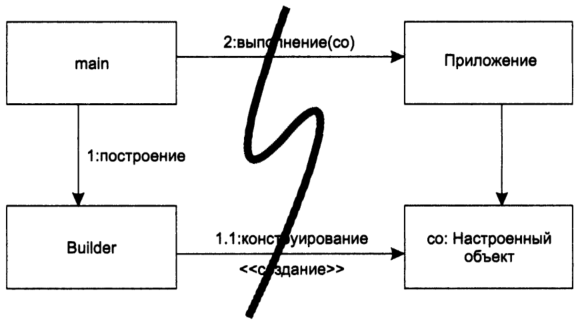
\includegraphics[width=0.4\textwidth]{builder.png}
                \end{center}
            \item Паттерн ``Factory'':
                \begin{center}
                    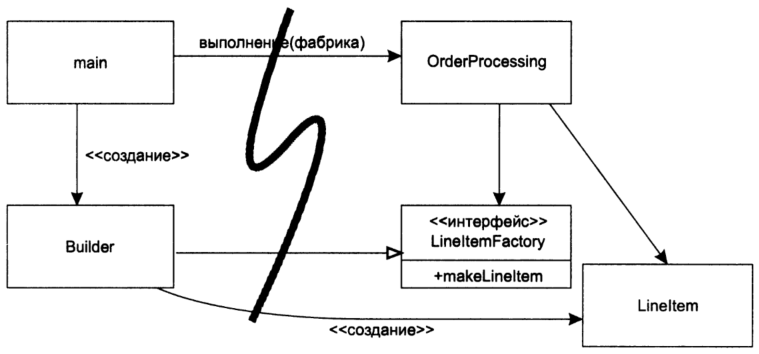
\includegraphics[width=0.4\textwidth]{factory.png}
                    \attribution{Р. Мартин, Чистый код}
                \end{center}
        \end{itemize}
    \end{frame}

    \begin{frame}
        \frametitle{Dependency Injection}
        \begin{itemize}
            \item Объект не должен создавать другие объекты, если только он не предназначен специально для этого
            \item Инициализация системы --- ответственность main или специального \textit{контейнера}
            \item Бюджетный способ --- реестр объектов

                \mintinline{java}|MyService myService = | \\
                \mintinline{java}|    (MyService)(jndiContext.lookup("NameOfMyService"));|
        \end{itemize}
    \end{frame}

    \begin{frame}
        \frametitle{Пример IoC-контейнера: Spring}
        \begin{center}
            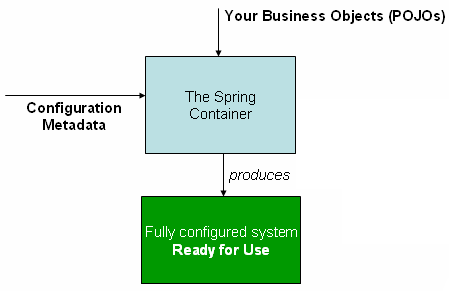
\includegraphics[width=0.5\textwidth]{springIoC.png}
        \end{center}
    \end{frame}

    \begin{frame}[fragile]
        \frametitle{Пример}
        \framesubtitle{Стековый калькулятор}
        \begin{small}
            \begin{minted}{java}
package ru.compscicenter.ioc;

public class Calculator {

    private Stack stack;

    public Calculator(Stack stack) {
        this.stack = stack;
    }

    public double calculate(String expression) {
        ...
        return stack.pop();
    }
}
            \end{minted}
        \end{small}
    \end{frame}

    \begin{frame}[fragile]
        \frametitle{Пример}
        \framesubtitle{Стек}
        \begin{minted}{java}
public interface Stack {
    void push(double value);
    double pop();
    boolean isEmpty();
}

public class LinkedStack implements Stack {
    ...
    ...
}
        \end{minted}
    \end{frame}

    \begin{frame}[fragile]
        \frametitle{Пример}
        \framesubtitle{Конфигурация контейнера}
        \begin{minted}{xml}
<?xml version="1.0" encoding="UTF-8"?>
<beans ....>

    <bean id="stack"
          class="ru.compscicenter.ioc.LinkedStack"
          />

    <bean id="calculator"
          class="ru.compscicenter.ioc.Calculator">
        <constructor-arg ref="stack"/>
    </bean>

</beans>
        \end{minted}
    \end{frame}

    \begin{frame}[fragile]
        \frametitle{Пример}
        \framesubtitle{main}
        \begin{minted}{java}
public class Main {
    public static void main(String[] args) {
        ApplicationContext context = 
            new FileSystemXmlApplicationContext("config.xml");

        Calculator calculator = 
            context.getBean("calculator", Calculator.class);

        double result = calculator.calculate("1 2 + 3 *");
        System.out.println(result);
    }
}
        \end{minted}
    \end{frame}

    \section{Мутабельность}

    \begin{frame}
        \frametitle{Мутабельность}
        \textbf{Мутабельность} --- способность изменяться
        \begin{itemize}
            \item Запутывает поток данных
            \item Гонки
        \end{itemize}
        \vspace{3mm}
        Чтобы сделать класс немутабельным, надо:
        \begin{itemize}
            \item Не предоставлять методы, модифицирующие состояние
            \begin{itemize}
                \item Заменить их на методы, возвращающие копию
            \end{itemize}
            \item Не разрешать наследоваться от класса
            \item Сделать все поля константными
            \item Не давать никому ссылок на поля мутабельных типов
        \end{itemize}
        Всё должно быть немутабельно по умолчанию!
    \end{frame}

    \section{Оптимизация}

    \begin{frame}
        \frametitle{Про оптимизацию}
        Во имя эффективности (без обязательности ее достижения) делается больше вычислительных ошибок, чем по каким-либо иным причинам, включая непроходимую тупость. \newline
        -- William A. Wulf 
    
        \vspace{3mm}
        Мы обязаны забывать о мелких усовершенствованиях, ска­жем, на 97\% рабочего времени: опрометчивая оптимизация --- корень всех зол. \newline
        -- Donald E. Knuth
    
        \vspace{3mm}
        Что касается оптимизации, то мы следуем двум правилам: \newline
        Правило 1. Не делайте этого.  \newline
        Правило 2 (только для экспертов). Пока не делайте этого -- т.е. пока у вас нет абсолютно четкого, но неоптимизированного решения. \newline
        -- M. A. Jackson
    \end{frame}

    \section{Общие рекомендации}

    \begin{frame}
        \frametitle{Общие рекомендации}
        \begin{itemize}
            \item Fail Fast
            \begin{itemize}
                \item Не доверяйте параметрам, переданным извне
                \item assert-ы -- чем больше, тем лучше
            \end{itemize}
            \item Документируйте все открытые элементы API
            \begin{itemize}
                \item И заодно всё остальное, для тех, кто будет это сопровождать
                \item Предусловия и постусловия, исключения, потокобезопасность
            \end{itemize}
            \item Статические проверки и статический анализ лучше, чем проверки в рантайме
            \begin{itemize}
                \item Используйте систему типов по максимуму
            \end{itemize}
            \item Юнит-тесты
            \item Continious Integration
            \item Не надо бояться всё переписать
        \end{itemize}
    \end{frame}

    \begin{frame}
        \frametitle{Заключение}
        \begin{columns}
            \begin{column}{0.5\textwidth}
                \begin{center}
                    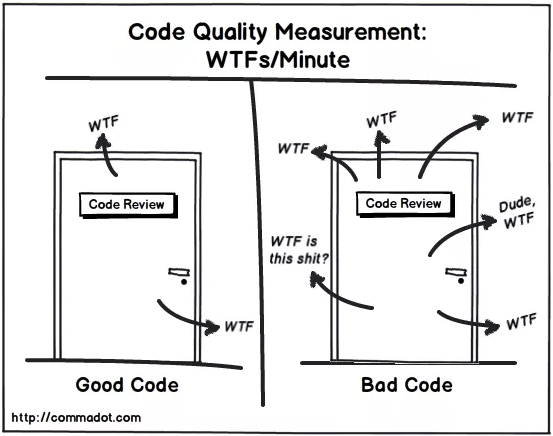
\includegraphics[width=0.7\textwidth]{wtfsMin.png}
                \end{center}
                \vspace{-0.8cm}
                \attribution{http://commadot.com, Thom Holwerda}
            \end{column}
            \begin{column}{0.5\textwidth}
                \begin{center}
                    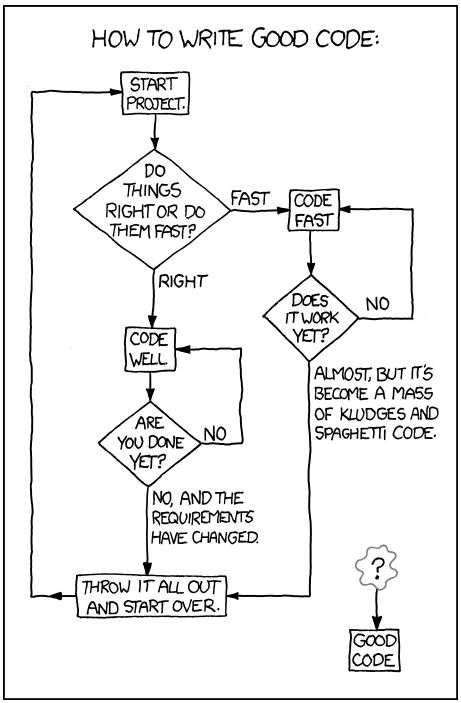
\includegraphics[width=0.7\textwidth]{goodCodeXkcd.png}
                \end{center}
                \vspace{-0.8cm}
                \attribution{https://xkcd.com}
            \end{column}
        \end{columns}
    \end{frame}

    \begin{frame}
        \frametitle{Книжки}
        \begin{columns}
            \begin{column}{0.5\textwidth}
                \begin{center}
                    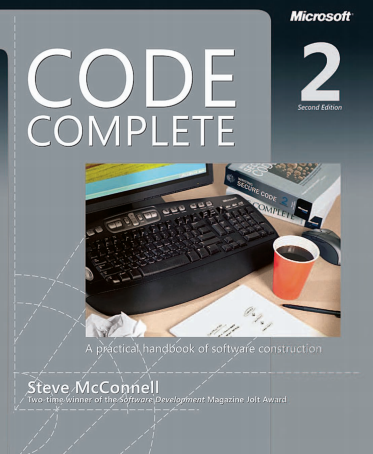
\includegraphics[width=0.5\textwidth]{codeCompleteCover.png}
                \end{center}
                \vspace{3mm}
                Steve McConnell, Code Complete
            \end{column}
            \begin{column}{0.5\textwidth}
                \begin{center}
                    
\includegraphics[width=0.5\textwidth]{cleanCodeCover.png}
                \end{center}
                \vspace{3mm}
                Роберт Мартин, Чистый Код
            \end{column}
        \end{columns}
    \end{frame}

\end{document}
